\section{Lab: System calls}

\subsection{实验目的}

本实验旨在进一步熟悉系统调用,重点掌握如何添加系统调用,理解系统调用的工作原理,内核态和用户态的联系。

本实验实现了两个系统调用:
\begin{itemize}
    \item System call tracing:实现对系统调用的跟踪;
    \item Sysinfo:收集有关正在运行的系统的信息。
\end{itemize}

\subsection{实验步骤}

\subsubsection{实现trace}

\begin{enumerate}
    \item 首先,根据提示,在Makefile的UPROGS中添加\$U/\_trace\textbackslash。
    \item 在user.h文件的system calls部分添加trace函数。
          \newpage
          \begin{lstlisting}[language=c, title=对user.h的改动]
    // system calls
    int fork(void);
    ...
    // 添加 trace函数
    int trace(int);
    \end{lstlisting}
    \item 在usys.pl末尾添加entry("trace");以便在汇编语言中添加这个函数。
    \item 进入kernel文件夹,在syscall.h中添加SYS\_trace系统调用号的定义,值往下类推,即为22。
          \begin{lstlisting}[language=c, title=对syscall.h的更改]
    // System call numbers
    #define SYS_fork 1
    ...
    // 为trace添加系统调用号
    #define SYS_trace 22
          \end{lstlisting}
    \item 更改进程结构体。在proc.h中的进程结构体最后添加一个掩码trace\_mask,用于记录哪些进程要被追踪。
          \begin{lstlisting}[language=c, title=对进程结构体的更改]
    struct proc
    {
        struct spinlock lock;
        ...
        // 添加掩码
        int trace_mask;
    };
    \end{lstlisting}
    \item 在sysproc.c文件中,添加系统调用函数sys\_trace,在调用时设置掩码。
          \begin{lstlisting}[language=c, title=实现sys\_trace系统调用]
    uint64 sys_trace(void)
    {
        // 获取参数
        int mask;
        if (argint(0, &mask) < 0)
            return -1;
        // 获取当前进程
        struct proc *p = myproc();
        // 写入掩码
        p->trace_mask = mask;
        return 0;
    }
    \end{lstlisting}
    \item 在syscall.c中修改syscall函数,使其根据掩码判断是否输出当前调用信息。
          \begin{lstlisting}[language=c, title=对syscall函数的修改]
    void syscall(void)
    {
        int num;
        struct proc *p = myproc();

        num = p->trapframe->a7;
        if (num > 0 && num < NELEM(syscalls) && syscalls[num])
        {
            p->trapframe->a0 = syscalls[num]();

            // 获得掩码
            int trace_mask = p->trace_mask;

            // 如果掩码对应,输出当前系统调用信息
            if ((trace_mask >> num) & 1)
            {
                printf("%d: syscall %s -> %d\n", 
                        p->pid, 
                        syscall_names[num - 1], 
                        p->trapframe->a0);
            }
        }
        else
        {
            ...
        }
    }
    \end{lstlisting}
    \item 修改proc.c中的freeproc函数和fork函数,确保掩码在进程释放时重置掩码、在子进程创建时传递掩码。
          \newpage
          \begin{lstlisting}[language=c, title=对proc.c的修改]
    static void freeproc(struct proc *p)
    {
        if (p->trapframe)
        kfree((void *)p->trapframe);
        ...

        // 添加了这一行
        p->trace_mask = 0;
    }

    int fork(void)
    {
        ...

        // 把子进程的掩码也设置为与父进程相同
        np->trace_mask = p->trace_mask;

        ...
    }
    \end{lstlisting}
\end{enumerate}

\subsubsection{实现sysinfo}
\begin{enumerate}
    \item 首先,先仿照trace中的方法,在Makefile、syscall.h、syscall.c、user.h、user.pl中注册名为sysinfo的系统调用。
    \item 在kalloc.c中仿照kalloc函数读取空闲内存链表的方式,实现一个计算空闲内存空间大小的函数acquire\_freeman。
          \begin{lstlisting}[language=c, title=acquire\_freemem的实现]
    uint64 acquire_freemem()
    {
        struct run *r;
        uint64 cnt = 0;

        // 锁
        acquire(&kmem.lock);
        r = kmem.freelist;
        // 遍历链表
        while (r)
        {
            r = r->next;
            cnt++;
        }
        // 释放锁
        release(&kmem.lock);
        // 返回空间大小(页数乘页尺寸)
        return cnt * PGSIZE;
    }
    \end{lstlisting}
    \item 在proc.c中,实现一个计算非使用状态进程个数的函数acquire\_nproc,利用记录进程的数组struct proc proc[NPROC]。
          \begin{lstlisting}[language=c, title=acquire\_nproc的实现]
    uint64 acquire_nproc()
    {
        struct proc *p;
        int cnt = 0;
    
        for (p = proc; p < &proc[NPROC]; ++p)
        {
            acquire(&p->lock);
            if (p->state != UNUSED)
                cnt++;
            release(&p->lock);
        }
    
        return cnt;
    }    
    \end{lstlisting}
    \item 最后,在sysproc.c中完成sys\_sysinfo函数的实现。利用argaddr读取参数的地址,利用copyout对地址进行写入。
          \begin{lstlisting}[language=c, title=sys\_sysinfo的实现]
    uint64 sys_sysinfo(void)
    {
        struct sysinfo info;
        uint64 addr;
        struct proc *p = myproc();

        // 计算空闲进程数
        info.nproc = acquire_nproc();
        // 计算空闲内存数
        info.freemem = acquire_freemem();

        // 获取参数
        if (argaddr(0, &addr) < 0)
            return -1;
        // 写入结构体
        if (copyout(p->pagetable, addr, (char *)&info, sizeof(info)) < 0)
            return -1;
        return 0;
    }
    \end{lstlisting}
\end{enumerate}

\subsection{评测结果}
利用grade-lab-syscall脚本评测,得到评测结果如图\ref{fig:syscall}所示。
\begin{figure}[h]
    \centering
    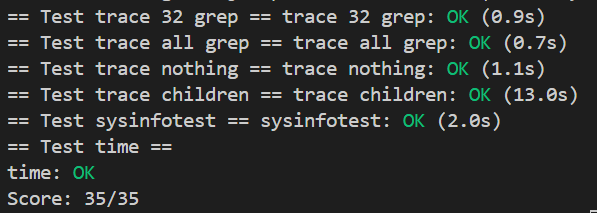
\includegraphics[width=\linewidth]{pics/syscall评测结果.png}
    \caption{评测结果}
    \label{fig:syscall}
\end{figure}

\subsection{实验小结}

在本实验中,我实现了两个系统调用。通过实验,我了解到了在内核中实现系统调用的一整套流程。

在实验中,为了实现我自己的系统调用,我阅读了许多kernel的代码,对内核有了更好的了解。通过仿照内核代码中一些函数的实现以及提示,我才得以完成我自己的系统调用。我在阅读内核代码的时候也遇到了一些困难,花费了不少时间来理解代码的含义。

这次实验大大加深了我对系统调用的了解,为之后的实验打下基础。
